%
% Chapter 6
%

\chapter{DATA AND MC SAMPLES}
This analysis is essentially a counting experiment that compares the number of \tth events predicted with the number of events observed after accounting for the backgrounds.
Simply put, this analysis compares the number of signal + background events predicted by MC to the number of events observed in real data, in the signal regions, after accounting for uncertainties. 
The hypothesis in this case is that the \tth process and all relevant\footnote{Here, relevant means any background capable of entering the signal regions.} backgrounds exist in the amounts dictated by
the Standard Model, and this hypothesis is represented by the MC. 

\section{Data samples}
The data in this analysis was collected from CMS throughout 2016 and only when the magnet was on\footnote{The CMS solenoid was notoriously problematic for datataking during 2015,
suffering from cryogenics issues related to the coldbox and rendering much of the data collected during that time useless from the perspective of most (but not all) physics analyses.}
and all subdetectors were fully operational.
The full 2016 dataset analyzed here corresponds to a total integrated luminosity of 35.9 fb$^{-1}$ and uses the single and double lepton datasets listed in table~\ref{tab:datasets}
and reconstructed with the \texttt{CMSSW\_8\_0\_x} software. This data corresponds to a center-of-mass energy of 13 TeV, and the spacing between bunches in the LHC was 25ns.
On average, there were 30 pileup events per bunch crossing in this data. This data was certified as ``good'' for data analysis internally by CMS~\cite{json}.
The global tags\footnote{The global tag is a CMS-specific parameter that automatically sets all subdetector alignment conditions and calibrations.} used to reconstruct and analyze this data are
\texttt{80X\_dataRun2\_2016SeptRepro\_v7}, corresponding to dataset eras B-G, and \texttt{80X\_dataRun2\_Prompt\_v16} corresponding to era H.

\begin{landscape}
%\setlength\LTcapwidth{5.5in}
%\begin{longtable}{lcp{4.5in}}
\begin{longtable}{p{4.5in}cr}
  \caption[DATA SAMPLES]{Datasets \label{tab:datasets} }\\
  \toprule
 Dataset & Run Range & Luminosity $\mathrm{fb}^{-1}$ \\

  \midrule
\endfirsthead
  \caption[]{{\em Continued}} \\  % Just like in Chp. 2
  \midrule
 Dataset & Run Range & Luminosity $\mathrm{fb}^{-1}$ \\
  \midrule
\endhead
\endfoot
  \bottomrule
\endlastfoot

\texttt{/SingleElectron/Run2016B-23Sep2016-v3/MINIAOD} & $273150$--$275376$ & $5.79$ \\
\texttt{/SingleElectron/Run2016C-23Sep2016-v1/MINIAOD} & $275656$--$276283$ & $2.57$ \\
\texttt{/SingleElectron/Run2016D-23Sep2016-v1/MINIAOD} & $276315$--$276811$ & $4.25$ \\
\texttt{/SingleElectron/Run2016E-23Sep2016-v1/MINIAOD} & $276831$--$277420$ & $4.01$ \\
\texttt{/SingleElectron/Run2016F-23Sep2016-v1/MINIAOD} & $277932$--$278808$ & $3.10$ \\
\texttt{/SingleElectron/Run2016G-23Sep2016-v1/MINIAOD} & $278820$--$280385$ & $7.54$ \\
\texttt{/SingleElectron/Run2016H-PromptReco-v2/MINIAOD} & $281207$--$284035$ & $8.39$ \\
\texttt{/SingleElectron/Run2016H-PromptReco-v3/MINIAOD} & $284036$--$284044$ & $0.22$ \\
\midrule
\texttt{/SingleMuon/Run2016B-23Sep2016-v3/MINIAOD} & $273150$--$275376$ & $5.79$ \\
\texttt{/SingleMuon/Run2016C-23Sep2016-v1/MINIAOD} & $275656$--$276283$ & $2.57$ \\
\texttt{/SingleMuon/Run2016D-23Sep2016-v1/MINIAOD} & $276315$--$276811$ & $4.25$ \\
\texttt{/SingleMuon/Run2016E-23Sep2016-v1/MINIAOD} & $276831$--$277420$ & $4.01$ \\
\texttt{/SingleMuon/Run2016F-23Sep2016-v1/MINIAOD} & $277932$--$278808$ & $3.10$ \\
\texttt{/SingleMuon/Run2016G-23Sep2016-v1/MINIAOD} & $278820$--$280385$ & $7.54$ \\
\texttt{/SingleMuon/Run2016H-PromptReco-v2/MINIAOD} & $281207$--$284035$ & $8.39$ \\
\texttt{/SingleMuon/Run2016H-PromptReco-v3/MINIAOD} & $284036$--$284044$ & $0.22$ \\
\midrule
\texttt{/DoubleEG/Run2016B-23Sep2016-v3/MINIAOD} & $273150$--$275376$ & $5.79$ \\
\texttt{/DoubleEG/Run2016C-23Sep2016-v1/MINIAOD} & $275656$--$276283$ & $2.57$ \\
\texttt{/DoubleEG/Run2016D-23Sep2016-v1/MINIAOD} & $276315$--$276811$ & $4.25$ \\
\texttt{/DoubleEG/Run2016E-23Sep2016-v1/MINIAOD} & $276831$--$277420$ & $4.01$ \\
\texttt{/DoubleEG/Run2016F-23Sep2016-v1/MINIAOD} & $277932$--$278808$ & $3.10$ \\
\texttt{/DoubleEG/Run2016G-23Sep2016-v1/MINIAOD} & $278820$--$280385$ & $7.54$ \\
\texttt{/DoubleEG/Run2016H-PromptReco-v2/MINIAOD} & $281207$--$284035$ & $8.39$ \\
\texttt{/DoubleEG/Run2016H-PromptReco-v3/MINIAOD} & $284036$--$284044$ & $0.22$ \\
\midrule
\texttt{/DoubleMuon/Run2016B-23Sep2016-v3/MINIAOD} & $273150$--$275376$ & $5.79$ \\
\texttt{/DoubleMuon/Run2016C-23Sep2016-v1/MINIAOD} & $275656$--$276283$ & $2.57$ \\
\texttt{/DoubleMuon/Run2016D-23Sep2016-v1/MINIAOD} & $276315$--$276811$ & $4.25$ \\
\texttt{/DoubleMuon/Run2016E-23Sep2016-v1/MINIAOD} & $276831$--$277420$ & $4.01$ \\
\texttt{/DoubleMuon/Run2016F-23Sep2016-v1/MINIAOD} & $277932$--$278808$ & $3.10$ \\
\texttt{/DoubleMuon/Run2016G-23Sep2016-v1/MINIAOD} & $278820$--$280385$ & $7.54$ \\
\texttt{/DoubleMuon/Run2016H-PromptReco-v2/MINIAOD} & $281207$--$284035$ & $8.39$ \\
\texttt{/DoubleMuon/Run2016H-PromptReco-v3/MINIAOD} & $284036$--$284044$ & $0.22$ \\
\midrule
\texttt{/MuonEG/Run2016B-23Sep2016-v3/MINIAOD} & $273150$--$275376$ & $5.79$ \\
\texttt{/MuonEG/Run2016C-23Sep2016-v1/MINIAOD} & $275656$--$276283$ & $2.57$ \\
\texttt{/MuonEG/Run2016D-23Sep2016-v1/MINIAOD} & $276315$--$276811$ & $4.25$ \\
\texttt{/MuonEG/Run2016E-23Sep2016-v1/MINIAOD} & $276831$--$277420$ & $4.01$ \\
\texttt{/MuonEG/Run2016F-23Sep2016-v1/MINIAOD} & $277932$--$278808$ & $3.10$ \\
\texttt{/MuonEG/Run2016G-23Sep2016-v1/MINIAOD} & $278820$--$280385$ & $7.54$ \\
\texttt{/MuonEG/Run2016H-PromptReco-v2/MINIAOD} & $281207$--$284035$ & $8.39$ \\
\texttt{/MuonEG/Run2016H-PromptReco-v3/MINIAOD} & $284036$--$284044$ & $0.22$ \\

\end{longtable}
\end{landscape}

\section{MC samples}


\subsection{Signal}
\subsection{Background}
\section{Triggers}


%% \begin{figure}[hbtp]
%%  \begin{center}
%%    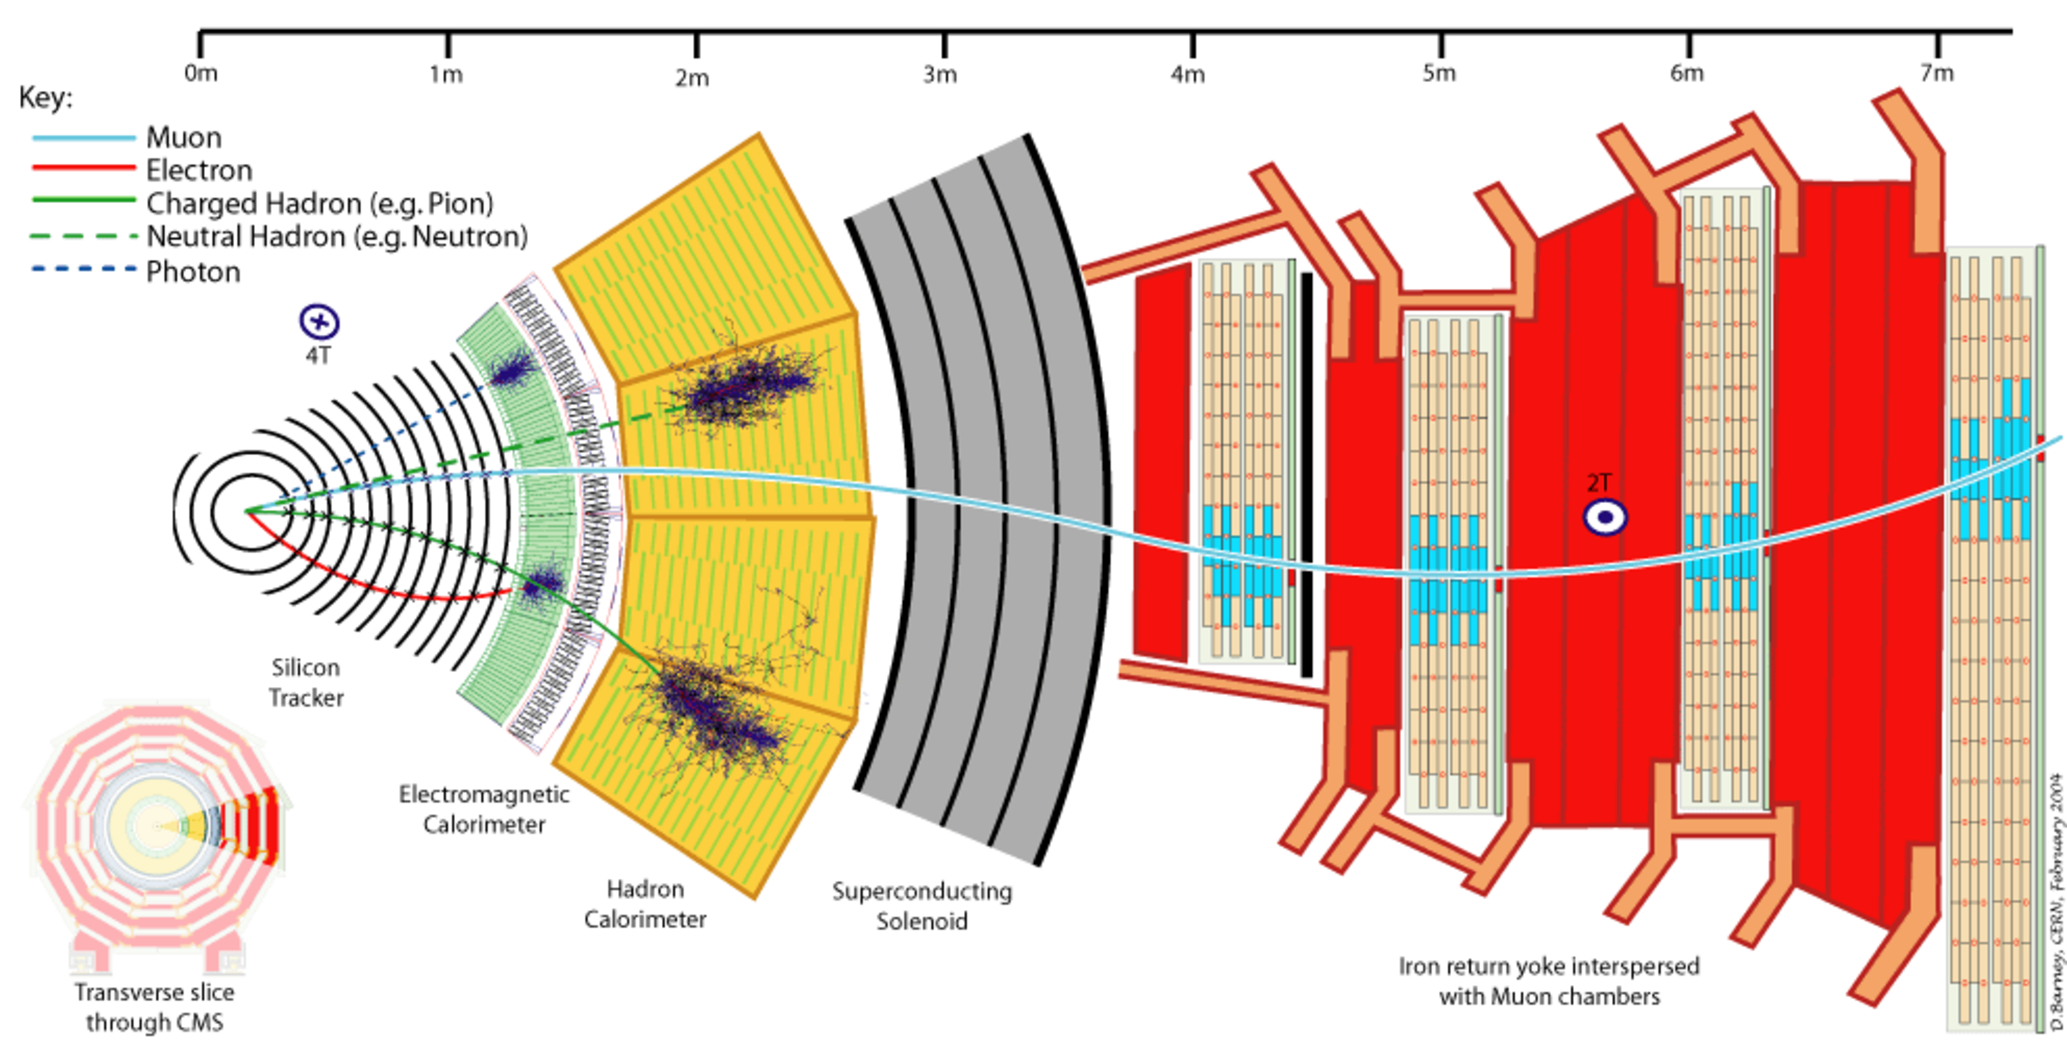
\includegraphics[width=0.8\textwidth]{ch4_figs/cms_particleflow.pdf}
%%    \caption{An overview of how CMS detects different types of particles. The slice of CMS in in the x-y plane.~\cite{NEED CITATION}.}
%%    \label{fig:cms_pflow}
%%  \end{center}
%% \end{figure}
